%%%%%%%%%%%%%%%%%%%%%%%%%%%%%%%%%%%%%%%%%%%%%%%%%%%%%%%%%%%%%
%% Begin exercise %%
%%%%%%%%%%%%%%%%%%%%%%%%%%%%%%%%%%%%%%%%%%%%%%%%%%%%%%%%%%%%%
\ex{High-frequency windings and planar transformers}

%%%%%%%%%%%%%%%%%%%%%%%%%%%%%%%%%%%%%%%%%%%%%%%%%%%%%%%%%%%%%
%% Task 1 %%
%%%%%%%%%%%%%%%%%%%%%%%%%%%%%%%%%%%%%%%%%%%%%%%%%%%%%%%%%%%%%

\task{Skin depth and Dowell's factor}

The windings are made of copper at $\SI{100}{\celsius}$, $\rho=\SI{2.26\cdot10^{-8}}{\ohm\metre}$. Dowell's factor for a winding of $M$ layers carrying a sinusoidal current is
\begin{equation}
	F_\mathrm{R}=\varphi\left[G_1(\varphi)+\frac{2}{3}\left(M^2-1\right)\left(G_1(\varphi)-2G_2(\varphi)\right)\right]
\end{equation}
with $\varphi=h/\delta$ and
\begin{equation}
	G_1=\frac{\sinh2\varphi+\sin2\varphi}{\cosh2\varphi-\cos2\varphi},\qquad G_2=\frac{\sinh\varphi\cos\varphi+\cosh\varphi\sin\varphi}{\cosh2\varphi-\cos2\varphi}.
\end{equation}

\subtask{Calculate the skin depth at 1, 2, 6.78 and $\SI{13.56}{\mega\hertz}$.}

\begin{solutionblock}
	$\delta=\sqrt{\rho/(\pi f\mu_0)}$: $\SI{75.7}{\micro\metre}$, $\SI{53.5}{\micro\metre}$, $\SI{29.1}{\micro\metre}$ and $\SI{20.5}{\micro\metre}$. At $\SI{20}{\celsius}$ the values are 13\,\% smaller.
\end{solutionblock}

\subtask{A planar winding has $M=4$ layers of $\SI{35}{\micro\metre}$ copper and carries a sinusoidal current at $\SI{2}{\mega\hertz}$. Calculate $\varphi$, $G_1$, $G_2$ and $F_\mathrm{R}$.}

\begin{solutionblock}
	$\varphi=35/53.5=0.654$, $G_1=1.5536$, $G_2=0.7536$, $G_1-2G_2=0.0463$:
	\begin{equation}
		F_\mathrm{R}=0.654\cdot\left(1.5536+\frac{2}{3}\cdot15\cdot0.0463\right)=1.32.
	\end{equation}
	The difference $G_1-2G_2$ is small: calculate with four digits.
\end{solutionblock}

\subtask{Find the optimum layer thickness at $\SI{2}{\mega\hertz}$ for $M=1$, 2 and 4.}

\begin{solutionblock}
	$M=1$: $\varphi_\mathrm{opt}=\pi/2$, $h=\SI{84}{\micro\metre}$. $M\geq2$: $\varphi_\mathrm{opt}\approx(15/(5M^2-1))^{1/4}$: $M=2$: 0.94, $h=\SI{50}{\micro\metre}$; $M=4$: 0.66, $h=\SI{35}{\micro\metre}$. In each case $F_\mathrm{R}\approx1.34$ to 1.44 at the optimum.
\end{solutionblock}

\subtask{Implement $F_\mathrm{R}(\varphi,M)$, find the optimum thickness numerically and compare it with the approximation (notebook).}

\begin{solutionblock}
	For $M\geq2$ the approximation is within 2\,\% of the numerical optimum, and $F_\mathrm{R}(\varphi_\mathrm{opt})=1.34$ to 1.35. For $M=1$ the optimum is $\varphi=\pi/2$ with $F_\mathrm{R}=1.44$.
\end{solutionblock}

%%%%%%%%%%%%%%%%%%%%%%%%%%%%%%%%%%%%%%%%%%%%%%%%%%%%%%%%%%%%%
%% Task 2 %%
%%%%%%%%%%%%%%%%%%%%%%%%%%%%%%%%%%%%%%%%%%%%%%%%%%%%%%%%%%%%%

\task{Winding of a ZVS buck inductor}

The inductor of brief B1 (Tutorial 6, Task 4) carries $I_\mathrm{dc}=\SI{8.33}{\ampere}$ plus a triangular ripple of $\Delta i=\SI{20}{\ampere}$ peak to peak at $\SI{2}{\mega\hertz}$; the current rises during $D=0.25$ of the period. The winding has $M=2$ layers. For $\SI{35}{\micro\metre}$ copper its DC resistance is $\SI{4}{\milli\ohm}$; it scales with $1/h$. The harmonic amplitudes of the triangle are
\begin{equation}
	\hat{\imath}_n=\frac{\Delta i\,|\sin(n\pi D)|}{\pi^2n^2D(1-D)}.
\end{equation}
Values of $F_\mathrm{R}$ for $M=2$:

\begin{center}
	\begin{tabular}{|l|c|c|c|c|c|c|}
		\hline
		$\varphi$           & 0.654 & 0.925 & 1.133 & 1.308 & 1.850 & 2.266 \\
		\hline
		$F_\mathrm{R}$      & 1.08  & 1.30  & 1.65  & 2.11  & 4.38  & 6.49  \\
		\hline
	\end{tabular}
	\captionof{table}{Dowell's factor for two layers}
	\label{tab:ex07_fr2}
\end{center}

\subtask{Calculate the rms value of the ripple and the rms values of the first three harmonics.}

\begin{solutionblock}
	$I_\mathrm{ac}=\Delta i/(2\sqrt{3})=\SI{5.77}{\ampere}$. Harmonic amplitudes 7.64, 2.70 and $\SI{0.85}{\ampere}$, i.e.\ rms values 5.40, 1.91 and $\SI{0.60}{\ampere}$. Together they contain 99.6\,\% of $I_\mathrm{ac}^2$.
\end{solutionblock}

\subtask{Estimate the winding loss for $\SI{35}{\micro\metre}$ and for $\SI{70}{\micro\metre}$ copper with the DC part and the first three harmonics.}

\begin{solutionblock}
	The $n$th harmonic sees $\varphi_n=\varphi_1\sqrt{n}$. $\SI{35}{\micro\metre}$ ($\varphi_1=0.654$):
	\begin{equation}
		P=\SI{4}{\milli\ohm}\cdot\left(8.33^2+5.40^2\cdot1.08+1.91^2\cdot1.30+0.60^2\cdot1.65\right)\si{\square\ampere}=\SI{4}{\milli\ohm}\cdot\SI{106.2}{\square\ampere}=\SI{0.42}{\watt}.
	\end{equation}
	$\SI{70}{\micro\metre}$ ($\varphi_1=1.308$, $R_\mathrm{dc}=\SI{2}{\milli\ohm}$):
	\begin{equation}
		P=\SI{2}{\milli\ohm}\cdot\left(69.4+29.2\cdot2.11+3.65\cdot4.38+0.36\cdot6.49\right)\si{\square\ampere}=\SI{2}{\milli\ohm}\cdot\SI{149.3}{\square\ampere}=\SI{0.30}{\watt}.
	\end{equation}
	The thicker copper loses 29\,\% less, although its $F_\mathrm{R}$ is much larger.
\end{solutionblock}

\subtask{Why is the best thickness larger here than for a purely sinusoidal current?}

\begin{solutionblock}
	Two thirds of $I_\mathrm{rms}^2$ is DC ($\SI{69.4}{\square\ampere}$ of $\SI{102.8}{\square\ampere}$), which sees only $R_\mathrm{dc}\propto1/h$. For the ripple alone the optimum would be about $\SI{47}{\micro\metre}$; with the DC part it moves to about $\SI{69}{\micro\metre}$. The waveform, including its DC part, decides the thickness.
\end{solutionblock}

\subtask{Calculate the loss with all harmonics for copper thicknesses from 10 to $\SI{250}{\micro\metre}$ and $M=1$, 2 and 4 (notebook).}

\begin{solutionblock}
	$M=2$: optimum at about $\SI{69}{\micro\metre}$, 29\,\% below $\SI{35}{\micro\metre}$; $M=4$: about $\SI{44}{\micro\metre}$. With one layer the loss keeps falling with thickness up to $\SI{250}{\micro\metre}$: the field acts on one side only, and the DC part profits from every micrometre.
\end{solutionblock}

%%%%%%%%%%%%%%%%%%%%%%%%%%%%%%%%%%%%%%%%%%%%%%%%%%%%%%%%%%%%%
%% Task 3 %%
%%%%%%%%%%%%%%%%%%%%%%%%%%%%%%%%%%%%%%%%%%%%%%%%%%%%%%%%%%%%%

\task{Layer stack of a planar transformer}

The 4:1 transformer of brief B2 uses eight PCB layers (\autoref{fig:ex07_stack}): copper $t=\SI{35}{\micro\metre}$, insulation $s=\SI{0.1}{\milli\metre}$ ($\varepsilon_\mathrm{r}=4.4$) between all layers, mean turn length $\mathrm{MLT}=\SI{40}{\milli\metre}$, winding breadth $h_\mathrm{w}=\SI{8}{\milli\metre}$. Stack (a): four primary layers with one turn each in series, four secondary layers in parallel. Stack (b): two primary turns per layer, two layers in series and the two halves in parallel; four secondary layers in parallel.

%%%%%%%%%%%%%%%%%%%%%%%%%%%%%%%%%%%%%%%%%%%%%%%%%%%%%%%%%%%%%%%%%%%%%%%%%%
% Layer stacks of the planar transformer (Exercise 07, Task 3)
%%%%%%%%%%%%%%%%%%%%%%%%%%%%%%%%%%%%%%%%%%%%%%%%%%%%%%%%%%%%%%%%%%%%%%%%%%

\begin{figure}[htb]
	\begin{center}
		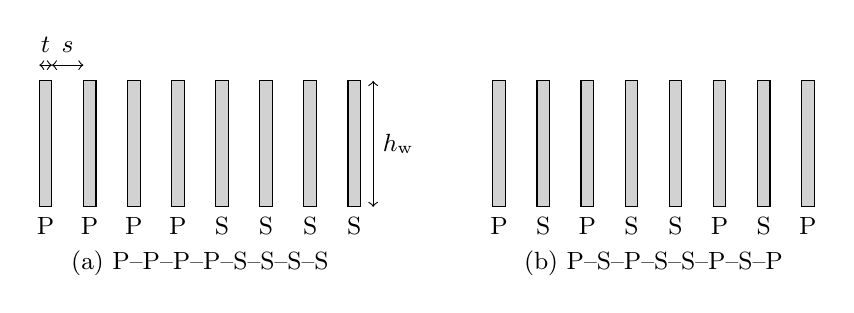
\begin{tikzpicture}[scale=0.8, every node/.style={font=\small}]
			% (a) PPPP-SSSS
			\foreach \k/\l in {0/P,1/P,2/P,3/P,4/S,5/S,6/S,7/S}{
					\fill[gray!35] (0.7*\k,0) rectangle (0.7*\k+0.2,2.0);
					\draw (0.7*\k,0) rectangle (0.7*\k+0.2,2.0);
					\node at (0.7*\k+0.1,-0.3) {\l};
				}
			\node at (2.55,-0.9) {(a) P--P--P--P--S--S--S--S};
			% dimensions
			\draw[<->] (0,2.25) -- (0.2,2.25);
			\node[anchor=south] at (0.1,2.3) {$t$};
			\draw[<->] (0.2,2.25) -- (0.7,2.25);
			\node[anchor=south] at (0.45,2.3) {$s$};
			\draw[<->] (5.3,0) -- (5.3,2.0) node[midway, right]{$h_\mathrm{w}$};
			% (b) PSPSSPSP
			\begin{scope}[xshift=7.2cm]
				\foreach \k/\l in {0/P,1/S,2/P,3/S,4/S,5/P,6/S,7/P}{
						\fill[gray!35] (0.7*\k,0) rectangle (0.7*\k+0.2,2.0);
						\draw (0.7*\k,0) rectangle (0.7*\k+0.2,2.0);
						\node at (0.7*\k+0.1,-0.3) {\l};
					}
				\node at (2.55,-0.9) {(b) P--S--P--S--S--P--S--P};
			\end{scope}
		\end{tikzpicture}
	\end{center}
	\caption{Cross-section of the two layer stacks (copper layers of thickness $t$, insulation $s$, winding breadth $h_\mathrm{w}$; not to scale)}
	\label{fig:ex07_stack}
\end{figure}


\subtask{Give the MMF at the layer boundaries, in units of the primary current $I_\mathrm{p}$, for both stacks.}

\begin{solutionblock}
	Every layer carries $I_\mathrm{p}$ ampere-turns in both stacks.\\
	(a): $0,1,2,3,4,3,2,1,0$.\\
	(b): $0,1,0,1,0,-1,0,-1,0$: the MMF never exceeds one layer's ampere-turns.
\end{solutionblock}

\subtask{Calculate the leakage inductance referred to the primary for both stacks with the 1-D energy method. Across a copper layer in which the MMF changes from $F_1$ to $F_2$: $\int F^2\mathrm{d}x=t(F_1^2+F_1F_2+F_2^2)/3$; across an insulation layer with constant $F$: $sF^2$; and $L_\mathrm{lk}=\mu_0\,\mathrm{MLT}/h_\mathrm{w}\cdot\int(F/I_\mathrm{p})^2\mathrm{d}x$.}

\begin{solutionblock}
	(a): copper layers $2\cdot(1+7+19+37)\,t/3=42.7\,t$, insulation $(1+4+9+16+9+4+1)\,s=44\,s$: $\int=\SI{5893}{\micro\metre}$,
	\begin{equation}
		L_\mathrm{lk}=\frac{\mu_0\cdot\SI{40}{\milli\metre}}{\SI{8}{\milli\metre}}\cdot\SI{5893}{\micro\metre}=\SI{37}{\nano\henry}.
	\end{equation}
	The formula with uniform current, $\mu_0N^2\mathrm{MLT}(d+(a+b)/3)/h_\mathrm{w}$ with $a=b=4t+3s=\SI{0.44}{\milli\metre}$ and $d=s$, gives $\SI{39.5}{\nano\henry}$.\\
	(b): copper $8\cdot t/3=2.7\,t$, insulation $4s$ (only the four P--S interfaces with $|F|=1$): $\int=\SI{493}{\micro\metre}$, $L_\mathrm{lk}=\SI{3.1}{\nano\henry}$, twelve times less.
\end{solutionblock}

\subtask{Calculate the capacitance per P--S interface and the total primary-to-secondary capacitance of both stacks. Estimate the common-mode current for an edge of $\SI{5}{\volt\per\nano\second}$.}

\begin{solutionblock}
	$C=\varepsilon_0\varepsilon_\mathrm{r}\,\mathrm{MLT}\,h_\mathrm{w}/s=\SI{125}{\pico\farad}$ per interface. (a) has one interface ($\SI{125}{\pico\farad}$), (b) six ($\SI{0.75}{\nano\farad}$). If the whole primary moved with $\SI{5}{\volt\per\nano\second}$ against the secondary: $\SI{0.62}{\ampere}$ and $\SI{3.7}{\ampere}$. This is an upper bound: the layers of a winding are at different potentials, and in a full bridge the edges of the two primary terminals partly cancel. Low leakage costs capacitance.
\end{solutionblock}

\subtask{Write a function for the leakage inductance of an arbitrary stack and evaluate also P--S--P--S--P--S--P--S. Plot the reduction of the leakage at high frequency, $L_\mathrm{lk,ac}/L_\mathrm{lk}$, versus $\Delta=h/\delta$ (notebook).}

\begin{solutionblock}
	37, 3.1 and $\SI{3.1}{\nano\henry}$: both interleaved stacks keep the MMF within one layer's ampere-turns, but P--S--P--S--P--S--P--S has seven P--S interfaces. With Hurley's expression the leakage stays within 3\,\% of its low-frequency value up to $\Delta=1$ and falls by 25 to 32\,\% at $\Delta=2$ (one to four layers).
\end{solutionblock}

%%%%%%%%%%%%%%%%%%%%%%%%%%%%%%%%%%%%%%%%%%%%%%%%%%%%%%%%%%%%%
%% Task 4 %%
%%%%%%%%%%%%%%%%%%%%%%%%%%%%%%%%%%%%%%%%%%%%%%%%%%%%%%%%%%%%%

\task{Winding capacitance and self-resonance}

An inductor of an EMI filter has $L=\SI{10}{\micro\henry}$ in two layers; the capacitance between the layers is $C_0=\SI{30}{\pico\farad}$.

\subtask{Calculate the winding capacitance and the self-resonance for a winding that goes back and forth, and for one in which both layers start at the same side.}

\begin{solutionblock}
	Back and forth: the voltage between the layers rises linearly from 0 to the full winding voltage $V$:
	\begin{equation}
		W=\frac{1}{2}C_0\frac{V^2}{3}\ \Rightarrow\ C_\mathrm{w}=\frac{C_0}{3}=\SI{10}{\pico\farad},\quad f_\mathrm{SRF}=\frac{1}{2\pi\sqrt{LC_\mathrm{w}}}=\SI{15.9}{\mega\hertz}.
	\end{equation}
	Same start side: constant voltage $V/2$ between the layers, $C_\mathrm{w}=C_0/4=\SI{7.5}{\pico\farad}$, $f_\mathrm{SRF}=\SI{18.4}{\mega\hertz}$; the return wire must cross the winding.
\end{solutionblock}

\subtask{The filter is used with a converter switching at $\SI{2}{\mega\hertz}$. Which harmonic lies at the self-resonance, and how could the self-resonance be raised?}

\begin{solutionblock}
	The 8th harmonic ($\SI{16}{\mega\hertz}$). Above $f_\mathrm{SRF}$ the inductor is capacitive and the filter loses attenuation. Higher $f_\mathrm{SRF}$: a single layer, sectioned windings, more distance between the layers, or two smaller inductors in series, each with its own lower capacitance.
\end{solutionblock}

%%%%%%%%%%%%%%%%%%%%%%%%%%%%%%%%%%%%%%%%%%%%%%%%%%%%%%%%%%%%%
%% Task 5 %%
%%%%%%%%%%%%%%%%%%%%%%%%%%%%%%%%%%%%%%%%%%%%%%%%%%%%%%%%%%%%%

\task{Winding concept of your brief (homework)}

Complete the magnetics part of milestone M1 (25.11.) with the windings.

\subtask{Choose the winding technology (PCB, foil, solid or litz wire, air core) and the number of layers for each magnetic component. Calculate $F_\mathrm{R}$ with the harmonics of your current waveform.}

\begin{solutionblock}
	Check list: skin depth at the operating temperature; number of layers $M$ from zero MMF to the MMF peak; thickness from the optimum for the actual waveform, including its DC part; terminations and vias.
\end{solutionblock}

\subtask{Estimate leakage inductance and winding capacitance and check them against the topology: resonant inductor, ZVS energy, self-resonance, common-mode current.}

\begin{solutionblock}
	The leakage follows from the 1-D energy method and must be checked at the operating frequency; the winding capacitance from the energy method; the inter-winding capacitance from the overlap area and the stack. A field-solver check (FEMM or FEMMT) is recommended before the layout (M2).
\end{solutionblock}

\vspace{0.5cm}
Remark: The notebook \texttt{tutorialEx07\_task.ipynb} evaluates Dowell's factor and the optimum thickness (Task 7.1), the harmonic loss of Task 7.2, the leakage and capacitance of arbitrary layer stacks (Task 7.3) and the self-resonance of Task 7.4.
